%Cancer has been at the forefront of biological and biomedical research for many years now, since it is one of the diseases still regarded as mostly uncurable. Since the advancements in biotechnology in the 1990s, producing enormous amounts of data, bioinformatics methods have played a crucial role in analyzing and interpreting this data.\\
In this chapter, we will first give a brief overview on the biology of cancer, specifically its formation and biological properties. For the characterization of these common properties, we will focus on the framework provided in the \textbf{Hallmarks Of Cancer}~\cite{hallmarks-of-cancer} by Hanahan and Weinberg in 2000. Then, we will introduce cancer cell lines as the model system we use for our analyses, as well as the methods for the characterization of cancer cell lines in regards to their biological properties and their response to various cancer drugs.\\
Given the vast diversity of cancer's biological properties~\cite{hallmarks-of-cancer,hallmarks_of_all_cancer_cells} across different cells, tumors and patients, a comprehensive understanding of cancer biology is both crucial for modern treatment approaches and challenging to achieve. The biological features of a tumor might have effects on all its behaviors, including but not limited to, aggressiveness, drug resistance, ability to develop metastasis, etc. After experimentally determining the drug sensitivity of cells using model systems such as cancer cell lines, finding analogies between the model and actual clinical patient cells is key for the transfer of this knowledge about drug response~\cite{cancer_cell_lines_useful_model}. Therefore, a detailed biological characterization of the cancer cell lines is essential.\\

\section{Cancer and its Formation}\label{sec:cancer_formation}
First, we will present a general introduction on cancer and the changes a healthy cell undergoes when it becomes cancerous. We will first focus on the information flow and gene expression in a healthy cell, after which we will underline what could go wrong in these processes and how that can lead to cancer.\\

\subsection{Information Flow in a Healthy Cell}\label{subsec:cf_info_healthy_cell}
%\textsc{DNA $\Rightarrow$ Transcription $\Rightarrow$ RNA $\Rightarrow$ Translation $\Rightarrow$ Protein}\\
%\textsc{Proteins play important roles in almost all essential processes in a cell.}\\
%As originally introduced by Francis Crick in 1958, the \emph{Central Dogma Of Biology} states that genetic information is passed down in a flow: It starts stored in form of a double-helix shaped molecule called \emph{DNA} (desoxyribonucleic acid), which is then \emph{transcribed} into the single-stranded \emph{RNA} (ribonucleic acid), which is in turn then \emph{translated} into \emph{proteins}, in a process called \emph{protein biosynthesis}\todo{mention that this is simplified, since gene expression does not only/necessarily yield proteins as a final result}. DNA and RNA primarily consist of a sequence of so-called nucleotide bases, the order of which encodes genetic information. The individual processes of \emph{transcription} and \emph{translation} are very complex, involving intricate molecular machinery and regulatory mechanisms to orchestrate gene expression and protein synthesis.\\

As introduced by Francis Crick in 1958, the \emph{Central Dogma Of Biology}~\cite{crick_central_dogma} states that genetic information is passed down in a flow. This model begins at the \emph{genome level}: the genetic information is stored in the nucleus of the cell in form of desoxyribonucleic acid (DNA), which is a double-stranded helix shaped molecule consisting primarily of 4 nucleotide bases, the order of which encodes genetic information. The process of transcription, where the DNA is used as a template to create the intermediate molecule RNA (ribonucleic acid), can be initiated by an enzyme called RNA polymerase.
%Many other molecules, called transcription factors, can facilitate or inhibit the transcription of DNA.
Many different kinds of RNA are synthesized in the cell, which fulfill a multitude of purposes, but here, we focus on messenger RNA (mRNA), which is later going to be translated into proteins. Once the RNA is synthesized, it goes through several post-processing steps\cite{molecular_cell_biology}, including but not limited to RNA splicing (cutting out sequences which should not be expressed from the RNA). All of the transcription machinery and processes can be summarized as the \emph{transcriptome level}.\\
Lastly, the mRNA is transported to the ribosomes, which are cell organelles where proteins are synthesized in a process known as \emph{translation}~\cite{molecular_cell_biology}. There, proteins are created by reading the RNA sequence and assembling a chain of amino acids, which becomes a protein after folding into an energetically favorable 3D conformation. The sequence of bases in the RNA determines which amino acid is synthesized, with each base triplet (group of three bases) encoding for one amino acid, as well as triplets to manage transcription more generally, like starting and stopping the transcription~\cite{spektrum_genetik}. Proteins can also undergo post-translational modifications, including changes to their structure and therefore function~\cite{molecular_cell_biology}.\\
%These processes are known as the \emph{proteome level}\todo{this is not clean.}.\\
Proteins play an important role in most cellular proceses.
%They are composed of a chain of amino acids and can take many different shapes and functions.
For every protein, its function is determined by its three-dimensional structure, as the conformation allows it to interact with other molecules~\cite{molecular_biology_of_the_cell}. In turn, the three-dimensional conformation of a protein is determined by the sequence of amino acids it is made of, as stated by \emph{Anfinsens Dogma}~\cite{anfinsens_dogma}. This implies that a single wrong nucleotide in the DNA can cause a defective RNA, which may cause a wrong amino acid and a malformed and defective protein.\\
Different types of proteins can take on different roles in the cell. For example, enzymes are proteins which catalyze chemical reactions in the cell, antibodies are proteins which are used by the immune system to fight foreign substances in the organism, and structural proteins provide structure, strength and shape to cells and organisms~\cite{molecular_cell_biology}.\\
The entire process of gene expression is higly regulated. It can be influenced by a multitude of factors, such as transcription factors (molecules that bind to the DNA and facilitate the binding of the RNA polymerase and the initiation of transcription). Another process regulating DNA expression involves epigenetic modifications~\cite{epigenetics_alternative_splicing,histone_exchange_transcription_regulation}. For instance, these include the binding of methyl groups onto the bases of the DNA (called \emph{methylation}), which temporarily prevent this section of DNA from being transcribed. Specifically, epigenetics is defined as ``the study of heritable changes in gene expression that occur independent of changes in the primary DNA sequence''~\cite{epigenetics_in_cancer}. Most commonly, these modifications lead to an alteration in gene expression of the concerned gene, or in a more extreme manner, gene silencing or activation, which can influence cellular processes further, such as modifying the immune response, drug response, or cause cancer development. The dense packing of the DNA in chromatin form is another aspect influencing its availability to be expressed, which can also be influenced by epigenetic influences~\cite{molecular_cell_biology}.\\
%Changes influencing the development of cancer are not limited to permanent changes to the genetic material itself, but can also include epigenetic changes. Epigenetics is currently defined as ``the study of heritable changes in gene expression that occur independent of changes in the primary DNA sequence''~\cite{epigenetics_in_cancer}. This includes, among others, modifications induced by environmental factors. For instance, epigenetic modifications can include DNA methylation, which can in turn facilitate or prevent the binding of transcription factors to the DNA, altering the gene expression. Modification of chromatin remodelling complexes, dysregulation of miRNAs and DNA hydroxymethylation are other possible epigenetic modifications, all of which ultimately may lead to alterations in gene expression, among other consequences.
%the order of which encodes the information and which biological products can be synthesized
%There are also many other types of proteins, all of which are still synthesized the same way and play various roles in the organism.\\
The diverse protein landscape also dictates the function of different cells. Since cells have different functions to fulfill depending on their type or localization (the microenvironment the cells are subjected to), the main way these differences manifest is through a different protein landscape being present in different cells~\cite{molecular_cell_biology}.\\
The previously metioned regulatory mechanisms are also responsible for regulating the differential gene expression according to the type of cell.\\

\subsection{Aberrations from the Typical Information Flow}\label{subsec:cf_aberrations}
While the typical information flow is a highly regulated process, with multiple layers of quality control and error detection and correction involved, errors and problems can still occur. These errors can include mistakes in the transcription process, where the RNA polymerase incorporates the wrong nucleotides while synthesizing the mRNA, which may lead to incorrect amino acids being incorporated and the resulting protein being defective. Furthermore, mistakes in RNA processing (e.g.\ splicing, where introns are removed from the transcribed mRNA) or during translation (misreading of the RNA sequence by the ribosome) can also happen.\\
Another kind of errors occurs when modifications in the DNA are not detected properly by the cell-internal DNA repair mechanisms. While DNA in itself is a very stable and reliable means of storing information~\cite{molecular_biology_of_the_cell}, errors still do occur. They can be caused by a multitude of different occurences, such as environmental factors (e.g. radiation damaging the DNA bases on a molecular level), or mistakes during the operation of cellular machinery on the DNA (replication, transcription, etc.). As the DNA undergoes many of these processes and may be subject to environmental influences at any time, the likelihood of errors remaining udetected by the repair mechanisms cannot be eliminated. A modification of DNA is called a \emph{mutation}.\\
The main issue caused by this instability and vulnerability is that errors in the DNA almost always have severe consequences~\cite{dna_instability}, as according to the \emph{Central Dogma Of Biology}, they propagate through the different layers of gene expression. One can clearly see how changes to the DNA will inevitably provoke changes in the biology of the cell.\\
%Epigenetic modifications (e.g. changes in methylation of the DNA, caused for example by environmental or lifestyle factors) can also strongly increase or decrease the expression of certain genes. Depending on the concerned gene, the consequences of such a change in expression can range from non-existent to dangerous and cancer-provoking.\\
A common type of consequence from changes to the DNA is a change in gene expression regulation. This is a factor very often observed in cancer cells, which differentiates them from healthy cells~\cite{molecular_cell_biology}. Some genes or biological processes might be \textit{over-expressed} in respect to healthy cells, while some others might be \textit{under-expressed}.\\
So-called cell cycle checkpoints regularly check the DNA for damage and trigger DNA repair mechanisms if necessary. If the damage is too great, they can also trigger an induced apoptosis (cell death)~\cite{dna_repair_genetic_instability_and_cancer}. Therefore, DNA repair mechanisms are inherently important to the survival of the cell, since defects in these processes can easily trigger medical conditions, such as cancer~\cite{dna_damage_cancer}.\\

\subsection{Cancer Formation}\label{subsec:cf_cancer_formation}
%{\color{red}
%New structure for this subsection:
%\begin{itemize}
%	\item definition of cancer
%	\item how does cancer form (aberrations in cells, gene expression, bypassing of control mechanisms)
%	\item hereditary and acquired aberrations
%	\item deregulation of cells $\Rightarrow$ nice transition into Hallmarks
%\end{itemize}
%Move things that regard biological aspects purely $($stability of DNA, mutations, etc$)$ into 2.1.2\\
%}
According to the United States National Cancer Institute, cancer is defined as ``a disease in which some of the body's cells grow uncontrollably and spread to other parts of the body''~\cite{nci_definition_cancer}. It has been a leading cause of death worldwide for many years, accounting for nearly one in six deaths in 2020~\cite{who-cancer}.\\
As discussed in Chapter~\ref{chapter:Intro}, cancer is usually caused by change in the biological activity in a cell. That change can be caused by different cellular events, like mutations, chromosomal abnormalities and many others.\\
%{\color{gray}In\todo{this line is about DNA stability $\Rightarrow$ put it into aberrations} isolation, DNA is a very stable and reliable way of storing information\addref{DNA stable}. However, with many processes occurring within the cell at all times, such as DNA reparation mechanisms, DNA replication or DNA transcription, there is always the possibility of errors. Such errors are one way to obtain \emph{mutations}\todo{move mutations to 2.1.2}, a modification of the DNA, changing the information stored. Those changes can have consequences, changing biological aspects and processes in the cell that are controlled by the DNA\todo{move consequences of mutations to 2.1.2}.\\
%Those mutations can sometimes remain silent, meaning they do not have any noticeable effect on the cell. However, mutations and their consequences can also have a beneficial or detrimental effect on the cell. One example for a mutation which would be beneficial to an individual cell would be the evasion of apoptosis. If the organism loses its ability to kill a defective cell in a controlled manner, the cell can grow uncontrollably.\\}
The mutations and aberrations from typical processes inside a cell might develop in the cell itself, or be inherited via cell multiplication from a previous generation of cells. The inheritance of modifications to the DNA allows mutations and modifications in general to accumulate over generations of cells. While one modification might not have any consequences for the survival and proliferation of the cell, the accumulation might have severe consequences and ultimately can facilitate the development of cancer~\cite{stem_cell_mutations}.\\
Some genes play a special role in the development of cancer: Oncogenes are genes which have been found to be cancer-facilitating, so their activation facilitates the formation and proliferation of tumors. Tumor-suppressing genes are genes which are typically activated in healthy cells and actively suppress tumor formation, so silencing of those genes would facilitate cancer formation~\cite{weinberg_biology_of_cancer}. Copy Number Alterations (CNAs), gene expression alterations or silencers (which repress gene expression) and promoters (which facilitate gene expression) are just some ways how an oncogene or a tumor-suppressing gene can be amplified or suppressed, allowing or disallowing it from fulfilling its effect. Mutations, especially loss of function mutations, can have a similar effect~\cite{introduction_to_genetic_analysis}.\\
The quest to find specific properties or common alterations that lead to cancer development has been one of the focuses in oncology. One landmark in this research was presented in 2000: \textit{The Hallmarks of Cancer} by Hanahan and Weinberg~\cite{hallmarks-of-cancer}.
%\section{Biological Features}\remove{remove this section entirely?}
%\subsection{Gene Expression Alterations}
%\footnotesize{\textsc{Keep focus on gene expression alterations and only give a brief overview over other biological features}}\\
%In\todo{some of these informations belong into 2.1.2, such as defining over- and under-expression (since they are used earlier), but most of this is unimportant.} cancer cells, one of the changes that is often present and differentiates cancer cells from regular cells is an altered gene expression profile.
%Some genes are \emph{over-expressed}, meaning expressed more than in healthy cells, while some other genes are \emph{under-expressed}, meaning expressed less than in a typical healthy cell.\\
%The causes for these alterations are various, including genetic mutations, epigenetic modifications, copy number alterations, and many others.\\
%The consequences of these alterations are clearly very diverse and can be very far-reaching.
%The alterations in cancer can activate or deactivate the expression of genes (\emph{gene activation} and \emph{gene silencing}) and therefore turn on or off the production of proteins, which can dramatically alter the overall activity of the cell.
%Considering a more broad view of the entire cell, the consequences can include many aspects that facilitate the formation and proliferation of cancer cells. For example, they can include uncontrolled cell proliferation, an increased resistance to apoptosis, or genomic instability.
%\subsection{Other features}
%There are many other kinds of biological features that can be used to characterize a tumor.\\
%For example, cancers are often affected by mutations, especially in so-called oncogenes or tumor supressor genes, which are genes that have been found to play an important role in cancer formation.
%Oncogenes\todo{this is important and belongs into 2.1.after the definition of cancer} are genes which have been found to be cancer-facilitating, so their activation facilitates the formation and proliferation of tumors; while tumor-suppressing genes are genes which are typically activated in healthy cells and actively suppress tumor formation, so silencing of those genes would facilitate cancer formation. Copy Number Alterations (CNAs), which designate the amplification or deletion of a genomic region (e.g. a gene), are another way how an oncogene or a tumor-suppressing gene can be amplified or suppressed.\\
%Furthermore\todo{belongs into 2.1.2}, different epigenetic modifications can have consequences on the overall biological activity of the cell. For instance, they can influence DNA methylation, which can in turn facilitate or prevent the binding of transcription factors to the DNA, altering the gene expression. Modification of chromatin remodelling complexes, dysregulation of miRNAs and DNA hydroxymethylation are other possible epigenetic modifications, all of which ultimately may lead to alterations in gene expression, among other consequences.\\
%However, most of the potential modifications (mutations, epigenetic modifications, copy number alterations, \ldots) mostly have consequences on gene expression, so gene expression alterations remain the most fundamental and important features to consider.
\section{Hallmarks Of Cancer}\label{sec:hallmarks}
%One main challenge in cancer therapy is that cancer cells and their properties tend to differ strongly between different tumors, since the mutations which cause the cancer cells to differ from regular cells are inherently random.
%Therefore, there is a vast and diverse array of mutations\todo{not only mutations, but their consequences, in my case changes to gene expression profiles}, which can occur in a very varied manner between different tumors or patients.
%Considering the \emph{Central Dogma of Biology}, these mutations clearly change different biological aspects in a cell, such as gene expression (among other things like proteins being modified or misformed), which causes them to create a vast and diverse array of cells with different biological properties between different tumors or patients.\\
While cancer is a condition characterized by its predominant heterogeneity, some similarities and common traits can be identified between different tumors, as first done in 2000 in \textit{The Hallmarks of Cancer} by Hanahan and Weinberg~\cite{hallmarks-of-cancer} and later extended in 2011, now comprising ten characteristics that are hypothesized to be common among all human cancers~\cite{hallmarks-of-cancer-next-generation}.\\
These specific cancer-facilitating modifications can be summarized as each compromising one natural mechanism of the body for preventing uncontrolled growth and proliferation of a cell.
%For example, one of these hallmarks is the ability of a cell to evade apoptosis~\cite{hallmarks-of-cancer}. Quite clearly, the controlled killing of cells by apoptosis is an important part of the cancer defense machinery in a cell~\cite{apoptosis_in_cancer}; so, to be able to proliferate as a tumor, it is important for a cell to be able to evade apoptosis. Two other proposed hallmarks are the ability to be self-sufficient in growth signals~\cite{hallmarks-of-cancer}, as well as the insensitivity to anti-growth signals~\cite{hallmarks-of-cancer}. In a typical healthy cell, cell growth is strictly regulated, but for a cancer cell which wants to grow and proliferate as much as possible, it needs to be able so self-supply the signals needed to grow, as well as ignore the signals intended to make the cell stop growing.
%\color{gray}These specific\todo{don't describe the hallmarks this abstractly, use some concrete examples to intuitively understand what Hallmarks are and do.} cancer-facilitating modifications can be cataloged into different fundamental ways of function, each bypassing one cancer defense mechanism deeply engrained into the fundamental biology of each and every cell. Six fundamental hallmarks were identified, as well as two emerging hallmarks and two enabling characteristics, which are suspected to lead to the development of the proposed hallmarks\todo{detail level is bad. Irrelevant if they are "hallmarks" or "enabling characteristics", what's relevant is the way they function}.\color{black}
These hallmarks attempt to create a small set of underlying principles that allow cancer research to develop into a logical science. They presented the first ``organizing principle for rationalizing the complexities of neoplastic disease''~\cite{hallmarks-of-cancer-next-generation}.\\
The first of these hallmarks is that cancer cells are self-sufficient in growth signals. That means that they don't require external signals (by way of hormones, e.g.) to initiate cell growth; they either produce these signals themselves (through so-called \textit{autocrine signaling}), activate the growth pathway (that would usually be activated by the previously mentioned signals), or destroy the negative feedback loops in place to prevent excessive growth through these signals.\\
The second and third hallmarks are that cancer cells tend to be insensitive to anti-growth signals and apoptosis. Similarly to the previous hallmark, the cancer cell circumvents the typical mechanisms meant to avoid uncontrolled growth and abnormal proliferation of cells; or, in the case of apoptosis, the most drastic and last line of defense against abnormally proliferating cells, the induced cell death.\\
The next two hallmarks are related to the actual uncontrolled growth and multiplication of tumors and cancer cells. They describe the ability of cancer cells to replicate an unlimited number of times (whereas regular cells die after a certain number of divisions), as well as the sustained formation of new blood vessels (\textit{angiogenesis}) to ensure the needed supply of oxygen and nutrients for the growth of a tumor.\\
Finally, the last of the originally proposed hallmarks of cancer is the ability of cancer cells to break away from their original site or organ of origin to invade other surrounding tissue and spread all across the body in a process called \textit{metastasis}6. This is the consequence of cancer best known by laymen, and it is extremely dangerous for the health and survival of the patient, as it can lead to failure in any organ that it might reach. Often, metastasizing cancer turns out to be deadly~\cite{metastatic_survival}.\\
Since these hallmarks were introduced, a multitude of cancer drugs were specifically designed to target these hallmarks~\cite{hallmarks_therapeutic_targeting, drug_development_hallmarks}.\\
In 2011, Hanahan and Weinberg extended their Hallmarks framework to include several other aspects. However, for the purpose of this thesis, we will limit ourselves to discussing the original six hallmarks in-depth.\\
Even though more and more common characteristics are being found, cancer is still a highly heterogenous disease, which still poses a significant challenge to any therapy aspirations.

\section{Cancer Cell Lines}\label{sec:cancer_cell_lines}
Cancer cell lines, or immortalized cell lines, are a type of model organism widely used in cancer research.\\
They are a population of cancer cells, which have been immortalized (either by a mutation occuring naturally, or by a modification induced in a laboratory) and can therefore be grown for prolonged periods of time \textit{in vitro}. As opposed to \textit{stem cells}, which can also divide indefinitely, immortalized cells are not part of the natural development of an organism.\\
Cell lines are very commonly used in cancer research~\cite{cancer_cell_lines_useful_model}, since they provide many advantages for this purpose: due to their immortality, they are able to provide almost infinite biological material for experimental purposes. Moreover, libraries like the GDSC database~\cite{gdsc} or the Cancer Cell Line Encyclopedia~\cite{ccle} have been unanimously used for many years in research all around the world, and the cell lines contained in them are highly characterized and a very large amount of properties, such as gene expression, mutations, but also behaviors such as sensitivity to specific drugs, are very well-known and shared among researches all around the globe.\\
Due to their ease of use in a laboratory context and their molecular similarity to tumors, cancer cell lines are well suited for estimating the drug response of a tumor.\\
Cancer cell lines do, however, also have some drawbacks: since some cell lines have been used for many years now, they can still be subject to mutations, so their genome can slightly change over many years of using them. This implies that the cells used for a specific experiment might not habe the exact same characteristics as when the cell line was characterized and priorly used. More importantly, the image of the actual cancer from which the cell line was created provided by the cell line, might become less and less accurate, with both of them experiencing mutations and modifications independently from one another over the course of many years. For that purpose, a close eye needs to be kept on the state of cell lines, and they need to be replaced when they stray too far away from the current cancer landscape.\\

\section{Drug Sensitivity}\label{sec:drug_sensitivity}
In this section, we'll introduce the measures of drug sensitivity we need for our analyses, including how they are genereated, what options there are, and what the values express.\\

\subsection{Cell Viability Assay}\label{subsec:ds_cell_viability}
The measures of drug sensitivity needed for our analyses are typically generated in an experimental setting.\\
%The typical procedure for screening drug sensitivity involves putting cells from the cancer cell line culture in a plate and adding varying concentrations of a drug to that well of the plate. , exposing the cells to the drug and simulating the treatment of the tumor with the drug in a patient.\\After exposing the cells to the drug, some way of measuring the effect of the drug on the cells is needed. One way to do this is via a cell viability assay. The cell viability is the proportion of cells which is still alive after the treatment, compared to an untreated control sample. It can be measured in various ways, including mechanical activity, mobility, or metabolic activity. CellTiter-Glo, a very common viability assay, measures metabolic activity of cells by lysing the cells and measuring the amount of ATP present in the cell.\\This process is repeated for several different concentrations of the drug. With the datapoints given for the different concentrations, a dose-response curve is created using a statistical model.
The first step of performing a cell viability assay is to seed the cells into a titer plate. Typically, these plates have 96 wells, but bigger plates are also used. Next, the cells are exposed to the condition that is to be assessed, which in our case would be the drug. A portion of the wells will be exposed to the drug (called treatment wells), but some wells will remain with only the cells in them (called control wells). This is so that the cell survival can be compared at the end of the experiment.\\
After this, a reagent is added to the plate to allow the detection of the cell viability later. The plate is then incubated, such that the reagent can react with the cells. After a certain period of incubation, the signal specific to the viability reagent used is detected. Usually, those signals are absorbance, fluorescence or luminescence, depending on the assay performed and reactive agent used.\\
Finally, the signal is analyzed and the cell viability is calculated, according to the following formula:
\begin{align}
	\text{Cell viability (\%)} = \left(\frac{\text{Signal from treated sample}}{\text{Signal from control}}\right)\times 100
\end{align}
There are many different types of cell viability assays which are used a lot. They include, for instance, MTT assays (which use a specific dye which is reduced by metabolically active cells, and measure the absorbance of a specific wavelength of light), Resazurin assays (which also use a specific dye which is reduced by metabolically active cells, but measure either fluorescence or absorbance) and ATP-based luminescence assays (such as CellTiter-glo~\cite{celltiterglo}, which lyse the cells and measure ATP levels afterwards, reflecting the metabolic activity of the cells before the lysis).

\subsection{Dose-Response Curves}\label{subsec:ds_dose_response_curve}
When attempting to experimentally measure drug sensitivity for a specific drug and cell line, the ideal result would be a curve, typically of sigmoidal shape, which describes the effectiveness of the drug at any concentration. The drug concentration can typically be found on the x-axis of that curve, whereas the y-axis either denotes the inhibition of cell activity, or the viability (cell survival) observed in the cell. The first option results in a growing curve (the cell activity becomes more and more inhibited with a larger drug concentration), while the second option results in a falling curve (more and more cells die due to the drug activity).\\
%In both cases, the curve follows a sigmoidal shape, which is the typical shape for dose-response curves.
The dose-response curve is typically sigmoidal, which can be explained biologically: at low doses, the probability of a drug and target molecule randomly encountering and binding is low, so the activity remains minimal. As the concentration increases, more of the drug molecules bind to target molecules, making the response curve grow quicker. However, at some point, a saturation is reached, where all or nearly all target molecules have bound to a drug molecule and increasing the drug dose doesn't allow for more interaction. From this curve, multiple measures of drug response in the form of individual numbers can be obtained. We will now consider two options.

%\subsection{Drug Sensitivity Metrics}
%After understanding how to screen cell lines to their sensitivity to specific drugs, we now need to understand which measures or units we can use to quantify the %response of a certain cell line to the treatment with a certain drug.
\subsection{IC50}\label{subsec:ds_ic50}
The \textsc{IC50} value is a metric which is used to measure drug sensitivity. It is typically expressed as micromolar concentration. More specifically, it measures the potency of a drug to inhibit a specific biological process or function. It expresses the \textit{half-maximal inhibitory concentration}, so the concentration of the drug, for which the inhibition of the target biological process reaches half of its maximum, which is the point where the cell viability reaches $50\%$ in comparison to the control cells.
%It is usually measured \textit{in vitro}.
Considering the dose-response curve for a specific drug-cell lines combination, the IC50 value can be found on the concentration axis at the point where the cell viability reaches half of its maximum. A dose-response curve with the IC50 point highlighted can be found in Figure~\ref{fig:ic50}.
\begin{figure}
	\centering
	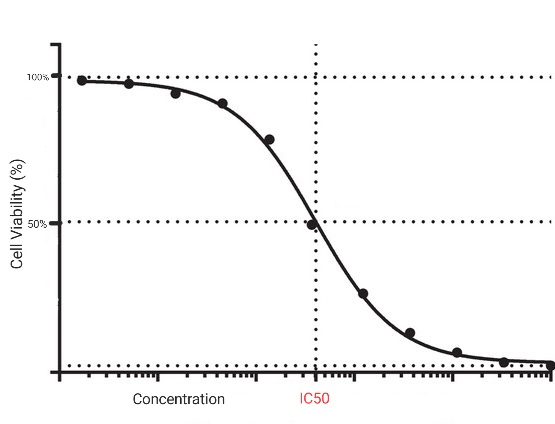
\includegraphics[width=0.7\textwidth]{IC50_dose_response.jpg}
	\caption{Dose-response curve with IC50 point highlighted}
	\label{fig:ic50}
\end{figure}
\subsection{CMax-Viability}\label{subsec:ds_cmax}
The \textsc{CMax-Viability} value is a different metric which also measures drug sensitivity. It was introduced in 2024 by Lenhof and Eckhart et al~\cite{cmax_viability}. It is typically expressed as either a numeric value between $0$ and $1$, which is what we used, or an equivalent percentage value between $0\%$ and $100\%$. It can be calculated from the same dose-response-curves as the \textsc{IC50}, it however expresses the drug sensitivity at a slightly different point in the drug-target interaction. Specifically, it expresses the cell viability (cell survival) at the peak concentration reached by the drug in the serum (\textsc{CMax}).
%It is similar to the \textsc{IC50} in that it expresses a value of drug sensitivity, but it differs in two specific aspects.
It expresses drug response by measuring the cell viability at a certain stage of drug concentration instead of expressing the drug concentration needed to reach a certain stage of inhibition, like an IC50 value would.
%Also, it considers the point of the dose-response curve where the concentration also reached by the maximum clinical dose~\cite{goodman_pharmacological_basis}, instead of the point of half inhibition considered by IC50.
Also, it focuses on the drug concentration achieved by the maximum clinical dose~\cite{goodman_pharmacological_basis}, rather than the IC50 point of half inhibition.
A dose-response curve visualizing the CMax-Viability value can be found in Figure~\ref{fig:cmax}.\\
As opposed to the more commonly used IC50 value, the CMax-Viability allows for a comparison between different drugs~\cite{cmax_viability}, since it considers only the maximum clinical concentration. The IC50 value is not comparable between drugs, since the clinical dose might differ very significantly from one drug to another. If the IC50 of a drug seems low, but the clinical dose is even lower, it might lead to false conclusions about practical drug sensitivity. Consequently, the CMax-Viability is much more useful for medical decision support.
\begin{figure}
	\centering
	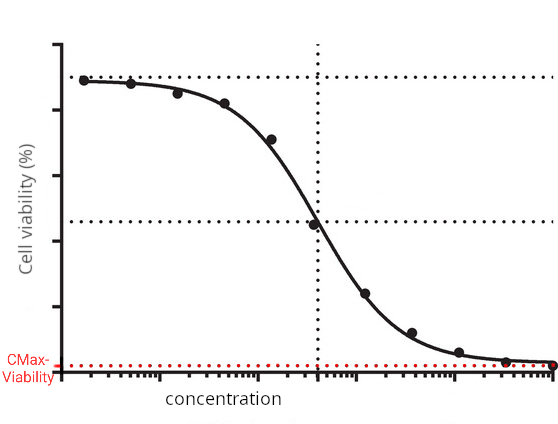
\includegraphics[width=0.7\textwidth]{CMax_viability_dose_response.png}
	\caption{Dose-response curve with CMax-Viability point highlighted}
	\label{fig:cmax}
\end{figure}
